Das Kameraobjektiv hat bestimmte Einstellungsmöglichkeiten, darunter die Blende und der Fokus.
Aufgrund der festen Brennweite des verwendeten Objektivs wird der Einfluss der Brennweite nicht genauer betrachtet.
Die entscheidenden Einstellungen für diesen Prozess sind also der Fokus und die Blende.
Über die Fokussteuerung kann eine einzelne Tiefenebene im Bild scharf gestellt werden.
Da das Prüfobjekt und das Streifenmuster in unterschiedlichen Tiefenebenen liegen, führt das bereits dazu, dass im Kamerabild nicht beides gleichzeitig fokussiert werden kann.
Der Fokus liegt zur Prüfung auf der Oberfläche des Objekts.
Dadurch wird das Streifenmuster unscharf, wodurch die Breiten der hellen und dunklen Streifen verändert werden.
Die zweite Einstellungsmöglichkeit ist die Blende.
Öffnet man diese weiter, lässt man mehr Licht in den Kamerasensor.
Durch mehr einfallendes Licht vergrößern sich die Breiten der hellen Streifen im Bild.
Oberflächendefekte des Prüfobjekts werden gleichzeitig besser sichtbar.
Zur Kompensation der unterschiedlichen Streifenbreiten im Kamerabild müssen die Breiten der hellen und dunklen Streifen im erzeugten Muster unterschiedlich gewählt werden (siehe Abbildung \ref{img:differenceCamPat}).

\begin{figure}[H]
	\centering
	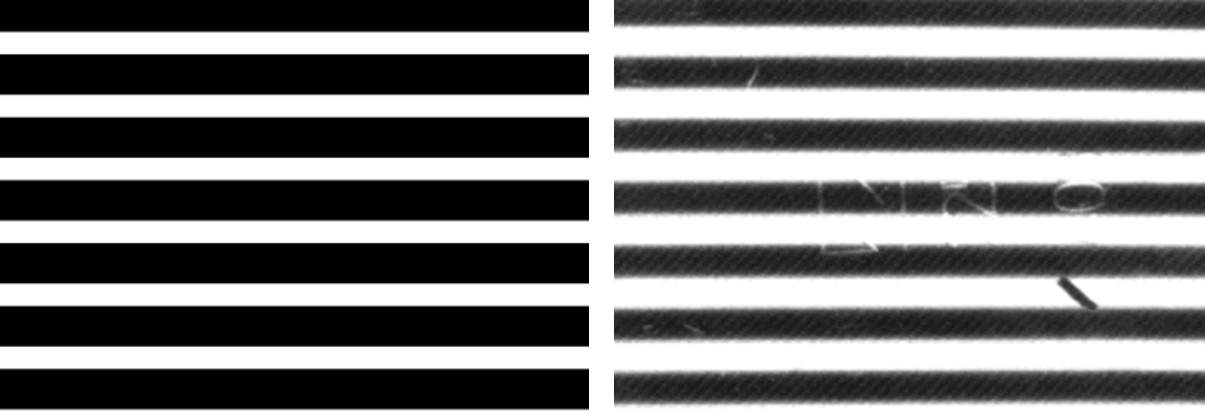
\includegraphics[width=\textwidth]{03_sichtpruefungDurchLichtstreuung/optimierungen/unterschiedeKameraUndMonitor/figures/differenceCameraPattern}
	\caption[Unterschied zwischen Muster und Kameraaufnahme]{Unterschied zwischen Muster und Kameraaufnahme. Links erzeugtes Muster mit fünf Pixel Breite der hellen und neun Pixel Breite der dunklen Streifen, rechts Kameraaufnahme}
	\label{img:differenceCamPat}
\end{figure}

\noindent
Man muss also mit Streifenmustern arbeiten, die von der Gleichung \ref{eq:rstreifenmuster} abweichen und unterschiedliche Breiten für die hellen und dunklen Streifen haben.
Es kommt dazu, dass die hellen und dunklen Streifen im Kamerabild unter Umständen nicht exakt gleich breit sein können, da die Anpassung der Streifenbreiten lediglich auf pixelgenauer Ebene durchgeführt werden kann.
Außerdem gibt es auch bei der Phase der Streifenmuster die Beschränkung, dass die maximale Genauigkeit der Verschiebung ein Pixel beträgt.
Das bedeutet, dass die Streifen selbst bei exakt gleicher Breite unter dem Kamerabild nicht genau versetzt zueinander liegen.
Es kommt hinzu, dass diese Genauigkeit sich auf den abbildenden Bildschirm bezieht.
Durch das Brillenglas zwischen der Kamera und dem Bildschirm kann die Phasenverschiebung im Kamerabild also mit zusätzlichen Fehlern behaftet sein.
Außerdem ist zu beachten, dass in der Kameraaufnahme stets ein Rauschen die Szene überlagert.